\documentclass[a4paper,10pt]{article}
\usepackage{mathtext}
\usepackage[T2A]{fontenc}
\usepackage[utf8]{inputenc}
\usepackage[russian]{babel}
\usepackage{amsmath}
\usepackage{amsfonts}
\usepackage{amssymb}
\usepackage{graphicx}
\usepackage[left=2cm,right=2cm,
    top=2cm,bottom=2cm,bindingoffset=0cm]{geometry}
\usepackage{color}
\usepackage{gensymb}

\usepackage{enumitem}
\setlist[enumerate]{label*=\arabic*.}

\usepackage{indentfirst}

\usepackage{titlesec}
\newcommand{\sectionbreak}{\clearpage}

%\graphicspath{ {<GraphicsPath>/} }
 
\begin{document}
\begin{titlepage}
  \begin{center}
    МОСКОВСКИЙ ГОСУДАРСТВЕННЫЙ УНИВЕРСИТЕТ \\ ИМ. Н.Э.БАУМАНА
    \vspace{0.25cm}
    
    Факультет "Энергомашиностроение"
    
    Кафедра "Э3"
    \vfill
    
    
    Жигалкин Александр Сергеевич
    \vfill

    \textsc{Курсовоей проект}\\[5mm]
    
    {\LARGE Проектирование свободной турбины ТВлД}
\end{center}
\vfill

\newlength{\ML}
\settowidth{\ML}{«\underline{\hspace{0.7cm}}» \underline{\hspace{2cm}}}
\hfill\begin{minipage}{0.4\textwidth}
  Руководитель курсового проекта\\
  \underline{\hspace{\ML}} В.\,Н.~Шадрин\\
  «\underline{\hspace{0.7cm}}» \underline{\hspace{2cm}} 2016 г.
\end{minipage}%
\bigskip

\vfill

\begin{center}
  Москва, 2016 г.
\end{center}
\end{titlepage}

\section{Задание}

Спроектировать двуступенчатую свободную турбину турбовального двигателя c температурой после камеры сгорания $T_г^*=1463\ К$ и мощностью на валу свободной турбины $N_e=2.07\ МВт$. 

\begin{figure}[hbtp]
\centering
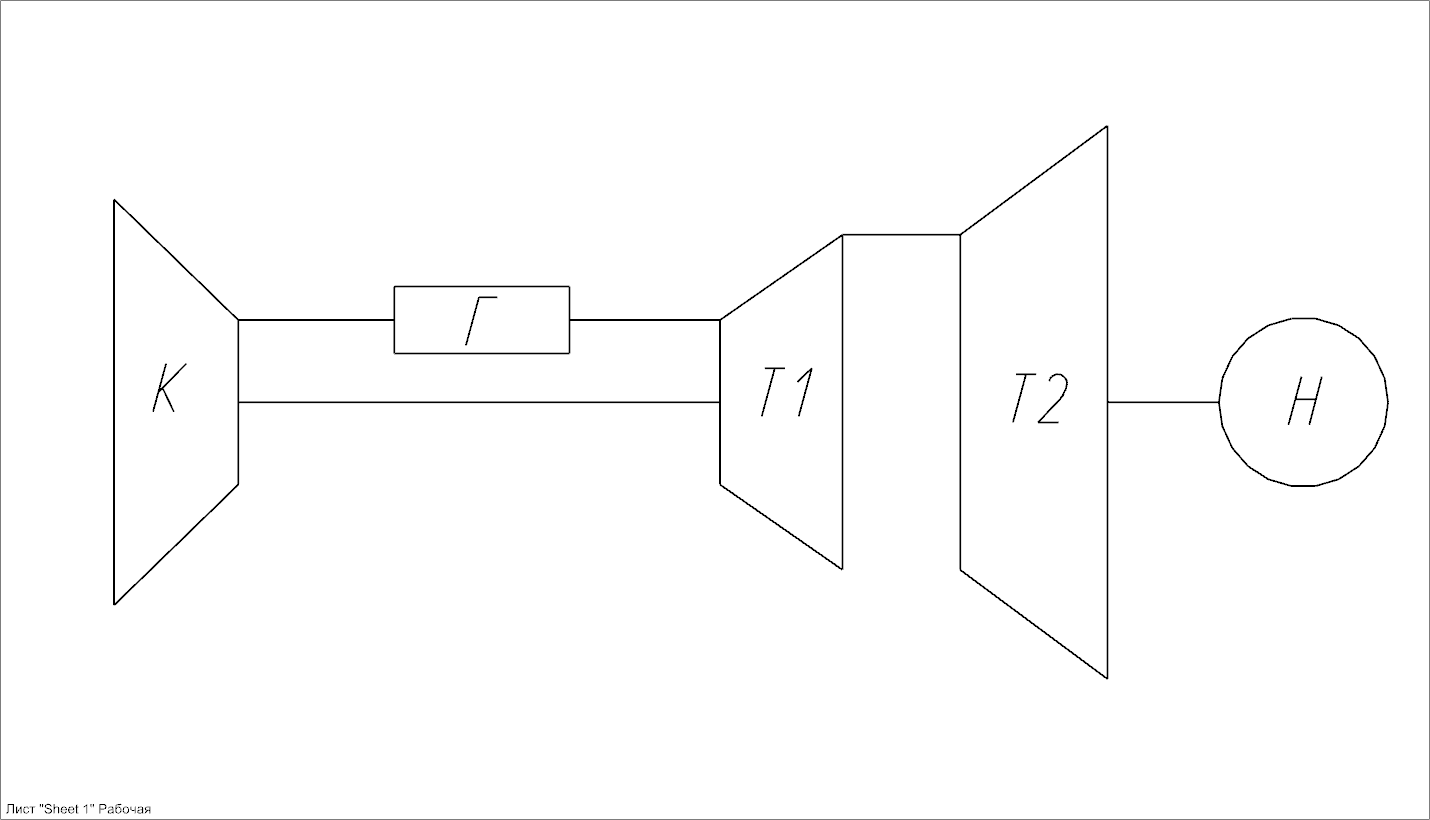
\includegraphics[scale=0.2]{../scheme.png}
\caption{Схема ГТД}
\end{figure}



\tableofcontents
\newpage

\section{Расчет параметров цикла ГТД}

\subsection{Исходные данные}
\begin{center}
	\begin{tabular}{|p{7cm}|c|c|c|}
		\hline
		\textbf{Величина} & \textbf{Обозначение} & \textbf{Размерность} & \textbf{Значение} \\ \hline
		Политропический КПД компрессора & $\eta_{кp}^*$ & - & <EtaCompPol> \\ \hline
		Полнота сгорания топлива & $\eta_г$ & - & <EtaBurn> \\ \hline
		Политропический КПД турбины компрессора & $\eta_{ткp}^*$ & - & <EtaCompTurbPol> \\ \hline
		Политропический КПД свободной турбины & $\eta_{тp}^*$ & - & <EtaFreeTurbPol> \\ \hline
		Относительная скорость на выходе из ГТД & $\lambda_{вых}$ & - & <LambdaOut> \\ \hline
		Мощность на валу свободной турбины & $N_e$ & кВт & <CyclePower> \\ \hline
		Температура перед турбиной компрессора & $T_г^*$ & К & <GasTemp> \\ \hline
		Коэффициент сохранения полного давления во входном устройстве компрессора & $\sigma_{вх}$ & - & <InletPipeSigma> \\ \hline
		Коэффициент сохранения полного давления в камере сгорания & $\sigma_{г}$ & - & <BurnSigma> \\ \hline
		Коэффициент сохранения полного давления в выходном патрубке & $\sigma_{вых}$ & - & <OutletPipeSigma> \\ \hline
		Механический КПД турбины компрессора & $\eta_м$ & - & <EtaMech> \\ \hline
		КПД редуктора & $\eta_р$ &  - & <EtaR> \\ \hline
		Относительный расход утечек & $g_{ут}$ &  - &<LossMassRateRel> \\ \hline
		Относительный расход на охлаждение & $g_{охл}$ &  - & <CoolMassRateRel> \\ \hline
		Относительный расход возвращаемого воздуха & $g_{возвр}$ & - & <ReturnMassRateRel> \\ \hline
	\end{tabular}
\end{center}

\subsection{Вариантные расчеты}
Для определения оптимальной степени повышения давления в компрессоре был произведен расчет цикла ГТД для различных значений  $\pi_к^*$ в интервале 6 до 27. В результате были построены графики зависимостей КПД, удельной расхода топлива и расхода через компрессор от степени повышения давления в компрессоре.

Ниже представлены графики зависимостей КПД, расхода топлива и расхода воздуха ГТД от $\pi_к^*$. Также представлен их сводный график, на котором для наглядности значения КПД, расхода топлива и расхода воздуха отнесены к максимальным на представленном промежутке значений степени повышения давления.

\begin{center}


	<CyclePlotGAir>	
	
	<CyclePlotCe>
	 
	<CyclePlotEtaE> 
\end{center}

\begin{figure}[hbtp]
\centering
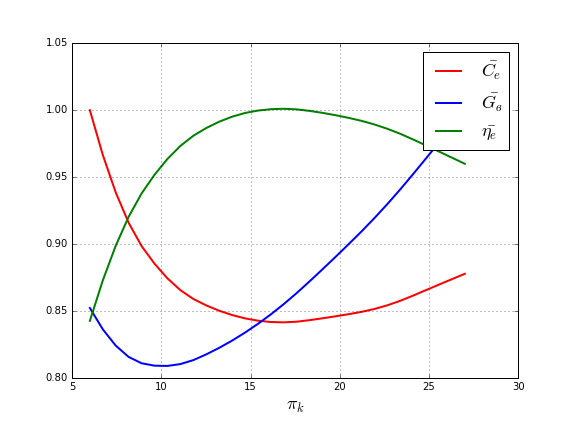
\includegraphics[scale=0.5]{../../plots/cycle_relative_quantities.png}
\caption{Сводный график зависимостей КПД, расхода воздуха и расхода топлива от степени повышения давления в компрессоре}
\end{figure}



В качестве оптимального принимаем $\pi_к = <PiComp>$.

Ниже представлен расчет цикла ГТД при $\pi_к = <PiComp>$

\subsection{Расчет цикла при $\pi_к = <PiComp>$}
Расчет некоторых узлов ГТД (а именно обоих турбин и компрессора) носит итерационный характер, так как удельная теплоемкость и коэффициент адиабаты зависят от температуры на выходе из узла. Поэтому ниже представлены расчеты для последних итераций.
\begin{enumerate}
	\item Определим давление за входным устройством: $$p_{вх}^* = \sigma_{вх} p_{а} = <InletPipeSigma> \cdot <AtmP> = <InletTubePOut> \/\ МПа$$
	\item Определим давление за компрессором: $$p_к^* = \pi_к p_{вх}^* = <PiComp> \cdot <InletTubePOut> = <CompPOut> \/\ МПа$$
	\item Определим адиабатический КПД компрессора, принимая показатель адиабаты воздуха $k_в = <CycleKAirShort>$: 
	\[\eta_{к}^* = \frac{\pi_к^{\frac{k_в - 1}{k_в} - 1}}
						{\pi_к^{\frac{k_в - 1}{k_в \eta_{кp}^* - 1}}} = 
		\frac{<PiComp>^{\frac{<CycleKAirShort> - 1}{<CycleKAirShort>} - 1}}
						{<PiComp>^{\frac{<CycleKAirShort> - 1}{<CycleKAirShort> \cdot <EtaCompPol> - 1}}} = <EtaComp>\]
	\item Определим температуру газа за компрессором: 
	$$T_к^* = T_a \left[ 1 + \frac{\pi_к^{\frac{k_в - 1}{k_в}} - 1}{\eta_к^*} \right] = 
	<AtmT> \left[ 1 + \frac{{<PiComp>}^{\frac{<CycleKAirShort> - 1}{<CycleKAirShort>}} - 1}{<EtaComp>} \right] = <CompTOut> \/\ К$$
	\item Определим уточненное значение показателя адиабаты:
	\begin{enumerate}
	
	\item Средняя теплоемкость воздуха при температуре $T_a$:
	\[c_{pв ср}(T_a) = \left( 1.2 \cdot 10^{-5} \left( T_a - 70 \right) + 0.236 \right) \cdot 4.187 \cdot 10^3 = \] 
	\[=\left( 1.2 \cdot 10^{-5} \left( <AtmT> - 70 \right) + 0.236 \right) \cdot 4.187 \cdot 10^3 =  <CompTInSpecificHeat>\ Дж / (кг \cdot К)
	\]
	\item Средняя теплоемкость воздуха при температуре $T_к^*$:
	\[c_{pв ср}(T_к^*) = \left( 1.2 \cdot 10^{-5} \left( T_a - 70 \right) + 0.236 \right) \cdot 4.187 \cdot 10^3 = \]
	\[=\left( 1.2 \cdot 10^{-5} \left( <CompTOut> - 70 \right) + 0.236 \right) \cdot 4.187 \cdot 10^3 =  <CompTOutSpecificHeat>\ Дж / (кг \cdot К)\]
	\item Cредняя теплоемкость воздуха в интервале температур от $T_a$ до $T_к^*$:
	\[c_{pв} = \frac{
	c_{pв ср}(T_к^*) (T_к^* - T_0) - c_{pв ср}(T_a)(T_a - T_0)
	}{
	T_к^* - T_a} = \]
	\[ =\frac{
	<CompTOutSpecificHeat> \cdot (<CompTOut> - <SpHeatT0>) - <CompTInSpecificHeat> \cdot (<AtmT> - <SpHeatT0>)
	}{
	<CompTOut> - <AtmT>} = <CycleAirSpecificHeat>\ Дж / (кг \cdot К)\]
	
	\item Новое значение показателя адиабаты:
	\[k_в^\prime = \frac{c_{pв}^\prime}{c_{pв}^\prime - R_в} = \frac{<CycleAirSpecificHeat>}{<CycleAirSpecificHeat> - <CycleAirGasConstant>} = <CycleKAirLong>\]
	\end{enumerate}
	
	\item Определим погрешность определения показателя адиабаты:
	$$\delta = \frac{\left| k_в^\prime - k_в \right|}{k_в} \cdot 100 \% = 
	\frac{\left| <CycleKAirLong> - <CycleKAirShort> \right|}{<CycleKAirShort>} \cdot 100 \% = 
	<CycleKAirDelta> \% < 5 \%$$
	Точность определения показателя адиабаты воздуха находится в пределах допуска.
	\item Используя найденный показатель адиабаты воздуха, определим теплоемкость воздуха в процессе сжатия воздуха в компрессоре:
	$$c_{pв} = \frac{k_в}{k_в - 1} R_в = 
	\frac{<CycleKAirShort>}{<CycleKAirShort> - 1} \cdot <CycleAirGasConstant> = 
	<CycleAirSpecificHeat> \/\ Дж/кг$$
	\item Определим работу компрессора:
	$$L_к = c_{pв} \left( T_к^* - T_a \right) = 
	<CycleAirSpecificHeat> \cdot \left( <CompTOut> - <AtmT> \right) = 
	<CompSpecificLabour> \cdot 10^6 \/\ Дж/кг $$
	\item Температура газа за камерой сгорания:
	$$T_г^* = <BurnerTOut> \/\ К$$
	\item Определим относительный расход топлива. Теплоемкость продуктов сгорания керосина рассчитывается через коэффициент избытка воздуха температуру. При расчета приняты следующие значения: 
	\begin{enumerate} % список значений для расчета удельного расхода топлива
		
		\item[1)] температура определения теплофизических параметров веществ: 
		$$T_0 = <ParameterDetermT> \/\ К;$$
		\item[2)] средняя теплоемкость воздуха перед камерой сгорания: 
		$$c_{pв}\left( T_к^* \right) = <BurnerInletAirSpecificHeat> \/\ Дж/(кг \cdot К);$$
		\item[3)] средняя теплоемкость чистых продуктов сгорания керосина после камеры сгорания: 
		\[c_{pг}\left( T_г^*,\ 1 \right) = \left[
		\frac{1.25 + 2.2}{10^5} (T_г^* + 450) + 0.218 
		\right]\cdot 4.187 \cdot 10^3 = \]
		\[=\left[
		\frac{1.25 + 2.2}{10^5} (<BurnerTOut> + 450) + 0.218 
		\right]\cdot 4.187 \cdot 10^3 = <BurnerOutletGasSpecificHeat> \/\ Дж/(кг \cdot К);\]
		\item[4)] средняя теплоемкость чистых продуктов сгорания керосина при температуре $T_0$: 
		\[c_{pг}\left( T_0,\ 1 \right) = \left[
		\frac{2.25 + 1.2}{10^5} (T_0 - 70) + 0.236 \right] \cdot 4.187 \cdot 10^3 = \]
		\[\left[
		\frac{2.25 + 1.2}{10^5} (<ParameterDetermT> - 70) + 0.236 \right] \cdot 4.187 \cdot 10^3 = 
		<ParameterDetermGasSpecificHeat> \/\ Дж/(кг \cdot К);\]
		\item[5)] низшая теплота сгорания топлива: $$Q_н^р = <LowerQ> \cdot 10^3 \/\ Дж / (кг \cdot К);$$
		\item[6)] полнота сгорания: $$\eta_г = <EtaBurn>;$$
		\item[7)] масса воздуха, необходимая для сжигания 1 кг топлива:
		$$l_0 = <TheoryAirMass> \/\ кг;$$
	\end{enumerate}

	\begin{enumerate}
		
		\item Определим относительный расход топлива:
		
		\[g_m = \frac{G_m}{G_в^г} = 
		\frac{
			c_{pг} \left( T_г^* \right) T_г^* - 
			c_{pв} \left( T_к^* \right) T_к^* 
		}{
			Q_н^р \eta_г - 
			\left[
				c_{pг} \left( T_г^* \right) T_г^* - 
				c_{pг} \left( T_0 \right) T_0 \right]	} =  \]
		\[=
		\frac{
			<BurnerOutletGasSpecificHeat> \cdot <BurnerTOut> - 
			<BurnerInletAirSpecificHeat> \cdot <CompTOut> 
		}{
			<LowerQ> \cdot 10^3 \cdot <EtaBurn> - 
			\left[
				<BurnerOutletGasSpecificHeat> \cdot <BurnerTOut> - 
				<ParameterDetermGasSpecificHeat> \cdot <ParameterDetermT>
			\right]		
		} = <FuelMassRateRel>\]
		
		\item Определим коэффициент избытка воздуха:
		$$\alpha = \frac{1}{g_m l_0} = 
		\frac{1}{<FuelMassRateRel> \cdot <TheoryAirMass>} = <CycleBurnAlphaLong>$$	
	\end{enumerate}
	
	\item Определим относительный расход газа:
		$$g_{г} = \left( 1 + g_m \right) \left( 1 - g_{ут} - g_{охл} \right) + g_{возвр} = 
		\left( 1 + <FuelMassRateRel> \right) \left( 1 - <LossMassRateRel> - <CoolMassRateRel> \right) + <ReturnMassRateRel> = <CompTurbineMassRateRel>$$
Расчет турбины компрессора состоит из двух частей. Первая часть - это определения температуры на выходе из турбины. Этот расчет является итерационным и ведется до сходимости по $k_г$.  Вторая часть - расчет давления торможения на выходе из турбины. Этот расчет также является итерационным и ведется до сходимости по $\pi_{тк}^*$. Ниже приведены последнии итерации обоих расчетов.	
	\item Определим удельную работу турбины компрессора:
	$$L_{тк} = \frac{L_к}{g_{г}\eta_м} = \frac{<CompSpecificLabour> \cdot 10^6}{<CompTurbineMassRateRel> \cdot <EtaMech> } = <CompTurbineSpecificLabour> \cdot 10^6 \/\ Дж/кг$$
	\item Определим давление газа перед турбиной компрессора:
	$$p_г^* = p_{к}^* \sigma_г = <CompPOut> \cdot <BurnSigma> = <CompTurbinePIn> \/\ МПа$$
	\item Определим среднюю теплоемкость газа в процессе расширения газа в турбине, принимая показатель адиабаты газа $k_г = <CycleCompTurbineKGasShort>$:
	$$c_{pг} = \frac{k_г}{k_г - 1} R_г = 
	\frac{<CycleCompTurbineKGasShort>}{<CycleCompTurbineKGasShort> - 1} \cdot <CycleCompTurbineGasConstant> = <CompTurbineSpecificHeat> \/\ Дж/(кг \cdot К) $$
	\item Определим температуру за турбиной компрессора:
	\[T_{тк}^* = T_г^* - \frac{L_{тк}}{c_{pг}} =
	<BurnerTOut> - \frac{<CompTurbineSpecificLabour> \cdot 10^6}{<CompTurbineSpecificHeat>} = <CompTurbineTOut>\]

	\item Определим уточненное значение показателя адиабаты газа:
	
	\begin{enumerate}
	\item Определим значение средней теплоемкости газа при температуре $T_{тк}^*$:
	\[c_{pг\ ср}(T_{тк}^*) = \left[ 
	\frac{1.25 +2.2 \alpha}{\alpha \cdot 10^5} (T_{тк}^* + 450) + 0.218
	\right] \cdot 4.187 \cdot 10^3= \]
	\[=\left[ 
	\frac{1.25 +2.2 \cdot <CycleBurnAlphaLong>}{<CycleBurnAlphaLong> \cdot 10^5} (<CompTurbineTOut> + 450) + 0.218
	\right] \cdot 4.187 \cdot 10^3= <CompTurbineTOutSpecificHeat>\ Дж / (кг \cdot К) \]
	\item Определим значение средней теплоемкости при температуре $T_г^*$:
	\[c_{pг\ ср}(T_г^*) = \left[ 
	\frac{1.25 +2.2 \alpha}{\alpha \cdot 10^5} (T_{тк}^* + 450) + 0.218
	\right] \cdot 4.187 \cdot 10^3= \]
	\[\left[ 
	\frac{1.25 +2.2 \cdot <CycleBurnAlphaLong>}{<CycleBurnAlphaLong> \cdot 10^5} (<CompTurbineTOut> + 450) + 0.218
	\right] \cdot 4.187 \cdot 10^3= <CompTurbineTInSpecificHeat>\ Дж / (кг \cdot К) \]
	\item Новое значение средней теплоемкости в интервале температур от $T_{тк}^*$ до $T_г^*$:
	\[c_{pг}^\prime = \frac{
	c_{pг\ ср}(T_г^*) (T_г^* - T_0) - c_{pг\ ср}(T_{тк}^*)(T_{тк}^* - T_0)
	}{
	T_{г}^* - T_{тк}^*} = \]
	\[=\frac{
	<CompTurbineTInSpecificHeat> \cdot (<BurnerTOut> - <SpHeatT0>) - <CompTurbineTOutSpecificHeat> \cdot (<CompTurbineTOut> - <SpHeatT0>)
	}{
	<BurnerTOut> - <CompTurbineTOut>} = <CompTurbineSpecificHeatLong>\ Дж / (кг \cdot К)\]
	\item Новое значение показателя адиабаты:
	\[k_в^\prime = \frac{c_{pг}^\prime}{c_{pг}^\prime - R_г} = \frac{<CompTurbineSpecificHeatLong>}{<CompTurbineSpecificHeatLong> - <CycleCompTurbineGasConstant>} = <CycleCompTurbineKGasLong>\]
	\end{enumerate}

	\item Определим погрешность определения показателя адиабаты:
	$$\delta = \frac{\left| k_г^\prime - k_г \right|}{k_г} \cdot 100 \% = 
	\frac{\left| <CycleCompTurbineKGasLong> - <CycleCompTurbineKGasShort> \right|}{<CycleCompTurbineKGasShort>} \cdot 100 \% = 
	<CompTurbineKCalcError> \% < 5 \%$$
	Погрешность определения показателя адиабаты в пределах допуска.
	\item Определим значение адиабатического КПД турбины компрессора, приняв степень понижения давления $\pi_{тк} = <CycleCompTurbinePiShort>$:
	\[\eta_{тк}^* = \frac{1 - \pi_{тк} ^ 
	                   {\frac{\left(1 - k_г \right) \eta_{ткp}^*}{k_г}}}
	              {1 - \pi_{тк} ^ 
	                   {\frac{1 - k_г}{k_г}} } = 
	          \frac{1 - <CycleCompTurbinePiShort> ^ 
	                   {\frac{\left(1 - <CycleCompTurbineKGasShort> \right) \cdot <EtaCompTurbPol>}{<CycleCompTurbineKGasShort>}}}
	              {1 - <CycleCompTurbinePiShort> ^ 
	                   {\frac{1 - <CycleCompTurbineKGasShort>}{<CycleCompTurbineKGasShort>}} } = <EtaCompTurb> \]	
	\item Определим давление воздуха за турбиной компрессора:
	$$p_{тк}^* = p_г^* 
	\left[ 
		1 - \frac{L_{тк}}{c_{pг} T_г^* \eta_{тк}^*}	
	\right] ^ \frac{k_г}{k_г - 1} = 	
	<CompTurbinePIn> 
	\left[ 
		1 - \frac{<CompTurbineSpecificLabour> \cdot 10^6}
		{<CompTurbineSpecificHeat> \cdot <BurnerTOut> \cdot <EtaCompTurb>}	
	\right] ^ \frac{<CycleCompTurbineKGasShort>}{<CycleCompTurbineKGasShort> - 1} =
	 <CompTurbinePOut> \/\ МПа$$
	 \item Определим новую степень понижения давления:
	 \[\pi_{тк}^{*\prime} = \frac{p_г^*}{p_{тк}^*} = \frac{<CompTurbinePIn>}{<CompTurbinePOut>} = <CycleCompTurbinePiLong>\]
	 \item Определим погрешность определения степени понижения давления:
	 $$\delta = \frac{\left| \pi_{тк}^{*\prime} - \pi_{тк}^* \right|}{\pi_{тк}^*} \cdot 100 \% = 
	\frac{\left| <CycleCompTurbinePiLong> - <CycleCompTurbinePiShort> \right|}{<CycleCompTurbinePiShort>} \cdot 100 \% = 
	<CompTurbinePiCalcError> \% < 5 \%$$
	Погрешность определения степени понижения давления в пределах допуска.
	
	
	\item Зададим значение приведенной скорости на выходе из выходного устройства:
	$$\lambda_{вых} = <LambdaOut>$$
	\item Определим давление торможения на выходе из выходного устройства, задавая показатель адиабаты газа $k_г = <CycleFreeTurbineKGasShort>$:
	$$p_{вых}^* = p_a \pi \left( \lambda_{вых}, k_г \right) = 
	<AtmP> \cdot \pi \left( <LambdaOut>, <CycleFreeTurbineKGasShort> \right) = 
	<OutletTubePOut> \/\ МПа$$

	\item Определим давление торможения за силовой турбиной:
	$$p_т^* = \frac{p_{вых}^*}{\sigma_{вых}} = \frac{<OutletTubePOut>}{<OutletPipeSigma>} = 
	<FreeTurbinePOut> \/\ МПа$$
	\item Определим степень понижения давления в силовой турбине:
	\[\pi_т = \frac{p_{тк}^*}{p_т^*} = \frac{<CompTurbinePOut>}{<FreeTurbinePOut>} = <FreeTurbinePi>\]
	\item Определим адиабатический КПД силовой турбины:
	\[\eta_{т}^* = \frac{1 - \pi_{т} ^ 
	                   {\frac{\left(1 - k_г \right) \eta_{тp}^*}{k_г}}}
	              {1 - \pi_{т} ^ 
	                   {\frac{1 - k_г}{k_г}} } = 
	          \frac{1 - <FreeTurbinePi> ^ 
	                   {\frac{\left(1 - <CycleFreeTurbineKGasShort> \right) <EtaFreeTurbPol>}{<CycleFreeTurbineKGasShort>}}}
	              {1 - <FreeTurbinePi> ^ 
	                   {\frac{1 - <CycleFreeTurbineKGasShort>}{<CycleFreeTurbineKGasShort>}} } = <EtaFreeTurb> \]	
	\item Определим температуру торможения на выходе из силовой турбины:
	$$T_т^* = T_{тк}^* 
	 \left\lbrace 
	 	1 - 
	 	\left[ 
	 		1 - 
	 			\left(
	 				\frac{p_{тк}^*}{p_т^*}
	 			\right) ^ \frac{k_г}{k_г - 1}
	 	\right] \eta_т^*
	 \right\rbrace = 
	 <CompTurbineTOut> 
	 \left\lbrace 
	 	1 - 
	 	\left[ 
	 		1 - 
	 			\left(
	 				\frac{<CompTurbinePOut>}{<FreeTurbinePOut>}
	 			\right) ^ \frac{<CycleFreeTurbineKGasShort>}{<CycleFreeTurbineKGasShort> - 1}
	 	\right] \cdot <EtaFreeTurb>
	 \right\rbrace = <FreeTurbineTOut> \/\ К$$
	 \item Определим уточненное значение показателя адиабаты газа в процессе расширения в силовой турбине:
		\begin{enumerate}
	\item Определим значение средней теплоемкости газа при температуре $T_{тк}^*$:
	\[c_{pг ср}(T_{тк}^*) = \left[ 
	\frac{1.25 +2.2 \alpha}{\alpha \cdot 10^5} (T_{тк}^* + 450) + 0.218
	\right] \cdot 4.187 \cdot 10^3= \]
	\[=\left[ 
	\frac{1.25 +2.2 \cdot <CycleBurnAlphaLong>}{<CycleBurnAlphaLong> \cdot 10^5} (<CompTurbineTOut> + 450) + 0.218
	\right] \cdot 4.187 \cdot 10^3= <CompTurbineTOutSpecificHeat>\ Дж / (кг \cdot К) \]
	\item Определим значение средней теплоемкости при температуре $T_т^*$:
	\[c_{pг ср}(T_т^*) = \left[ 
	\frac{1.25 +2.2 \alpha}{\alpha \cdot 10^5} (T_{тк}^* + 450) + 0.218
	\right] \cdot 4.187 \cdot 10^3= \]
	\[\left[ 
	\frac{1.25 +2.2 \cdot <CycleBurnAlphaLong>}{<CycleBurnAlphaLong> \cdot 10^5} (<CompTurbineTOut> + 450) + 0.218
	\right] \cdot 4.187 \cdot 10^3= <FreeTurbineTOutSpecificHeat>\ Дж / (кг \cdot К) \]
	\item Значение средней теплоемкости в интервале температур от $T_{т}^*$ до $T_{тк}^*$:
	\[c_{pг} = \frac{
	c_{pг ср}(T_{тк}^*) (T_{тк}^* - T_0) - c_{pг ср}(T_{т}^*)(T_{т}^* - T_0)
	}{
	T_{тк}^* - T_{т}^*} = \]
	\[\frac{
	<CompTurbineTOutSpecificHeat> \cdot (<CompTurbineTOut> - <SpHeatT0>) - <FreeTurbineTOutSpecificHeat> \cdot (<FreeTurbineTOut> - <SpHeatT0>)
	}{
	<CompTurbineTOut> - <FreeTurbineTOut>} = <FreeTurbineSpecificHeat>\ Дж / (кг \cdot К)\]
	\item Новое значение показателя адиабаты:
	\[k_в^\prime = \frac{c_{pг}}{c_{pг} - R_г} = \frac{<CompTurbineSpecificHeatLong>}{<CompTurbineSpecificHeatLong> - <CycleCompTurbineGasConstant>} = <CycleFreeTurbineKGasLong>\]
	\end{enumerate}	 

	\item Определим погрешность определения показателя адиабаты газа в процессе расширения в силовой турбине:
	$$\delta = \frac{\left| k_г^\prime - k_г \right|}{k_г} \cdot 100 \% = 
	\frac{\left| <CycleFreeTurbineKGasLong> - <CycleFreeTurbineKGasShort> \right|}{<CycleFreeTurbineKGasShort>} \cdot 100 \% = 
	<FreeTurbineKCalcError> \% < 5 \%$$
	Погрешность определения показателя адиабаты в пределах допуска.
	\item Определим значение теплоемкости газа в свободной турбине:
	$$c_{pг} = \frac{k_г}{k_г - 1} R_г = 
	\frac{<CycleFreeTurbineKGasShort>}{<CycleFreeTurbineKGasShort> - 1} \cdot <CycleFreeTurbineGasGasConstant> = <FreeTurbineSpecificHeat> Дж/(кг \cdot К)$$
	\item Определим удельную работу силовой турбины:
	$$L_т = c_{pг} \cdot \left( T_{тк}^* - T_т^* \right) = 
	<FreeTurbineSpecificHeat> \left( <CompTurbineTOut> - <FreeTurbineTOut> \right) = 
	<FreeTurbineSpecificLabour> \cdot 10^6 Дж/кг$$
	\item Определим удельную мощность ГТД:
	$$N_{e уд} = L_т g_г \eta_м \eta_р = 
	<FreeTurbineSpecificLabour> \cdot 10^6 \cdot <FreeTurbineMassRateRel> <EtaMech> <EtaR> = 
	<EngineSpecificPower> \cdot 10^6 Дж/кг$$
	\item Определим экономичность ГТД:
	$$C_e = \frac{3600}{N_{e уд}} g_т \left(1 - g_{охл}
	- g_{ут}\right) = 
	\frac{3600}{<EngineSpecificPower> \cdot 10^6} \cdot <FuelMassRateRel> \cdot \left(1 - <CoolMassRateRel>
	- <LossMassRateRel>\right) = 
	<EngineFuelMassRateSpecific> \cdot 10^{-3} кг/\left( Вт \cdot ч \right)$$
	\item Определим КПД ГТД:
	$$\eta_e = \frac{3600}{C_e Q_н^р} = 
	\frac{3600}{<EngineFuelMassRateSpecific> \cdot 10^{-3} \cdot <LowerQ> \cdot 10^6} 
	= <EngineEta>$$
	\item Определим расход воздуха:
	$$G_в = \frac{N_e}{N_{e уд} } = 
	\frac{<CyclePower> \cdot 10^3}{<EngineSpecificPower> \cdot 10^6 } = 
	<EngineMassRate> кг/с$$
\end{enumerate}


\section{Поступенчатый расчет турбины}
\subsection{Расчет первой ступени}
Исходные данные для расчета перовй ступени:

\begin{center}
	\begin{tabular}{|p{7cm}|c|c|c|}
		\hline
		\textbf{Величина} & \textbf{Обозначение} & \textbf{Размерность} & \textbf{Значение} \\ \hline
		Реактивность ступени & $\rho$ & - & $<Reactivity>$ \\ \hline
		Радиальный зазор & $\delta_r$ & - & $<DeltaR>$ \\ \hline
		Относительная длина лопатки статора & $\left( \frac{l}{D} \right)_1$ & - & $<StatorLRel>$ \\ \hline
		Удлинение лопатки статора & $\left( \frac{l}{b_a} \right)_{СА}$ & - & $<StatorElongation>$ \\ \hline 
		Удлинение лопатки ротора & $\left( \frac{l}{b_a} \right)_{РК}$ & - & $<RotorElongation>$ \\ \hline 
		Относительная ширина зазора между лопатками ротора и лопатками статора & $\left( \frac{\delta}{b_a} \right)_{СА}$ & - & $<StatorDeltaRel>$ \\ \hline
		Угол раскрытия на втулке & $\gamma_{вт}$ & \degree & $<GammaIn>$ \\ \hline
		Угол раскрытия на периферии & $\gamma_{пер}$ & \degree & $<GammaOut>$ \\ \hline
		Теплоперепад по статическим параметрам & $H_т$ & Дж/кг & $<Ht>$ \\ \hline
				
	\end{tabular}
\end{center}

\begin{enumerate}
	\item Определим теплоперепад на сопловом аппарате: 
	$$H_с = \left( 1 - \rho \right) H_т =
	\left( 1 - <Reactivity> \right) \cdot <Ht> \cdot 10^6 = <Hc> \cdot 10^6 \/\ Дж/кг$$
	\item Примем коэффициент адиабаты равным: $k_г = <St1KGasShort>$
	\item Теплоемкость газа при данном значении коэффициента адиабаты:
	\[c_{pг} = \frac{k_г R_г}{k_г - 1} = \frac{<St1KGasShort> \cdot
	<St1GasConstant>}{<St1KGasShort> - 1} = <St1SpecificHeat>\ Дж / (кг \cdot К)\]
	\item Определим действительную скорость истечения из СА:
	$$c_1 = \phi \sqrt{2 H_с} = 
	<Phi> \cdot\sqrt{2 <Hc> \cdot 10^6}  = <C1> \/\ м/с$$
	\item Определим температуру на выходе из СА:
	$$T_1 = T_0^* - \frac{c_1^2}{2c_{pг}} = 
	<St1GasTemp> - \frac{{<C1>}^2}{2 \cdot <St1SpecificHeat>} = <T1> \/\ К$$
	\item Определим температуру конца адиабатного расширения:
	$$T_1^\prime = T_0^* - \frac{H_c}{c_{pг}} = 
	<St1GasTemp> - \frac{<Hc>\cdot 10^6}{<St1SpecificHeat>} = <T1Prime> \/\ К$$
	\item Определим давление на выходе из СА:
	$$p_1 = p_0^* \left( \frac{T_1^\prime}{T_0^*} \right)^\frac{k_г}{k_г - 1} = 
	<St1PIn> \cdot \left( \frac{<T1Prime>}{<St1GasTemp>} \right)^\frac{<St1KGasShort>}{<St1KGasShort> - 1} = <P1> \/\ МПа$$
	\item Определим плотность газа на выходе из СА:
	$$\rho_1 = \frac{p_1}{R_г T_1} = 
	\frac{<P1> \cdot 10^6}{<St1GasConstant> \cdot <T1>} = <Rho1> \/\ кг/м^3$$
	\item Зададим угол на выходе из СА:
	$$\alpha_1 = <Alpha1> \degree$$
	\item Определим осевую скорость на выходе из СА:
	$$c_{1a} = c_1 \cdot \sin \alpha_1 = 
	{<C1> \cdot \sin<Alpha1>\degree} = <C1a> \/\ м/с$$
	\item Определим площадь на выходе из СА:
	$$A_1 = \frac{G}{c_{1a} \rho_1} = 
	\frac{<G>}{<C1a> \cdot <Rho1>} = <A1> \/\ м^2$$
	\item Определим средний диаметр турбины на выходе из СА:
	$$D_1 = \sqrt{
		\frac{A_1}{\pi \left( \frac{l}{D} \right)_1}
	} = \sqrt{
		\frac{<A1>}{\pi \cdot <StatorLRel>}
	} = <StatorDOut> \/\ м $$
	\item Определим окружную скорость на среднем диаметре на входе в РК:
	$$u_1 = \frac{\pi D_1 n}{60} = \frac{\pi \cdot <RotorDIn> \cdot <RotationSpeed>}{60} = <U1> \/\ м/с$$
	\item Определим относительную скорость на входе в РК:
	$$w_1 = \sqrt{c_1^2 + u_1^2 - 2 c_1 u_1 \cos \alpha_1} = 
	\sqrt{{<C1>}^2 + {<U1>}^2 - 2 \cdot <C1> \cdot <U1> \cdot \cos <Alpha1> \degree} = <W1> \/\ м/с$$
	
	 \item Определим теплоперепад на РК:
	 $$H_л = H_т \rho \frac{T_1}{T_1^\prime} = 
	 <Ht> \cdot 10^6 \cdot <Reactivity> \cdot \frac{<T1>}{<T1Prime>} = <Hl> \cdot 10^6 \/\ Дж/кг$$
	\item Определим осевую ширину рабочего колеса:
	\[b_{а\ рк} = \left( \frac{l}{b_a} \right)_{РК} 
	\frac{1}{1-\frac{\tan \gamma_п + \tan \gamma_в}{\left( \frac{l}{b_a} \right)_{РК} }} D_1 \left( \frac{l}{D} \right)_1 = 
	<RotorElongation>
	\frac{1}
	{1-\frac{\tan <GammaOut> + \tan <GammaIn>}
			{<RotorElongation>} }
	<StatorDOut> \cdot <StatorLRel> = <BaRK>\]
	
	 \item Определим средний диаметра на выходе из РК:
	 $$D_2 = D_1 + \frac{\tan \gamma_в - \tan \gamma_п}{2} b_{а\ рк} = 
	   		<StatorDOut> + \frac{\tan <GammaIn> \degree - \tan <GammaOut> \degree}{2} \cdot <BaRK> = 
	   		<RotorDOut> \/\ м$$
	 \item Определим длину лопатки на выходе из РК:
	 $$l_2 = D_1 \left( \frac{l}{D} \right)_1 + \frac{\tan \gamma_в + \tan \gamma_п}{2} b_{а\ рк} = 
	 		<StatorDOut> \cdot <StatorLRel> + \frac{\tan <GammaIn> \degree + \tan <GammaOut> \degree}{2} \cdot <BaRK> = 
	 		<L2> \/\ м$$
	 \item Определим относительную длину лопаток на выходе из РК:
	 $$\left( \frac{l}{D} \right)_2 = \frac{l_2}{D_2} = \frac{<L2>}{<RotorDOut>} = 
	 <RotorLRel>$$	 
	\item Определим площадь на выходе из РК:
	\[A_2 = \pi D_2 l_2 = \pi \cdot <RotorDOut> \cdot <L2> = <A2>\ м^2\]
	 \item Определим окружную скорость на среднем диаметре на выходе из РК:
	 $$u_2 = \frac{\pi D_2 n}{60} = \frac{\pi \cdot <RotorDOut> \cdot <RotationSpeed>}{60} = <U2> \/\ м/с$$
	 \item Определим относительную скорость истечения газа из РК:
	 $$w_2 = \psi \sqrt{w_1^2 + 2H_л +\left( u_2^2 - u_1^2 \right)} = 
	 <Psi> \cdot \sqrt{{<W1>}^2 + 2 \cdot <Hl> \cdot 10^6 +\left( {<U2>}^2 - {<U1>}^2 \right)} = <W2> \/\ м/с$$
	 \item Определим статическую температуру на выходе из РК:
	 $$T_2 = T_1 + \frac{
	 	\left( w_1^2  - w_2^2 \right) + \left( u_2^2 - u_1^2 \right)
	 }{2 c_{p г}} = 
	 <T1> + \frac{
	 	\left( {<W1>}^2  - {<W2>}^2 \right) + \left( {<U2>}^2 - {<U1>}^2 \right)
	 }{2 \cdot <St1SpecificHeat>} = <T2> \/\ К$$
	 \item Определим статическую температуру при адиабатическом процессе в РК:
	 $$T_2^\prime = T_1 - \frac{
	 	H_л
	 }{ c_{p г}} = 
	 <T1> - \frac{
	 	<Hl>\cdot 10^6
	 }{ \cdot <St1SpecificHeat>} = <T2Prime> \/\ К$$
	 \item Определим давление на выходе из РК:
	 $$p_2 = p_1 \left( \frac{T_2^\prime}{T_1} \right)^{\frac{k_г}{k_г - 1}} = 
	 <P1> \left( \frac{<T2Prime>}{<T1>} \right)^{\frac{<St1KGasShort>}{<St1KGasShort> - 1}} = <P2> \/\ МПа$$
	 \item Определим плотность газа на выходе из РК:
	 \[\rho_2 = \frac{p_2}{R T_2} = \frac{<P2> \cdot 10^6}{<St1GasConstant> \cdot <T2>} = <Rho2>\]
	 \item Определим осевую составляюшую абсолютной скорости на выходе из РК:
	 \[c_{2a} = \frac{G}{A_2 \rho_2} = \frac{<G>}{<A2> \cdot <Rho2>} = <C2a>\]
	 \item Определим угол в относительном движении на выходе из РК:
	 $$\beta_2 = \arcsin\frac{c_{2a}}{w_2} = \arcsin\frac{<C2a>}{<W2>} = <Beta2> \degree$$
	 \item Определим угол выхода из РК в абсолютном движении:
	 $$\alpha_2 = \arctan\frac{w_2 \cos \beta_2 - u_2}{c_{2a}} = 
	 \arctan\frac{<W2> \cdot \cos <Beta2> \degree - <U2>}{<C2a>} = <Alpha2> \degree$$
	 \item Определим окружную составляющую скорости на выходе из РК:
	 $$c_{2u} = w_2 \cos \beta_2 - u_2 = 
	 <W2> \cdot \cos <Beta2> \degree - <U2> = <C2u> \/\ м/с$$
	 \item Определим скорость потока на выходе из РК:
	 $$c_2 = \sqrt{c_{2u}^2 + c_{2a}^2} = \sqrt{{<C2u>}^2 + {<C2a>}^2} = <C2> \/\ м/с$$

	 \item Определим работу на окружности колеса:
	 $$L_u = c_{1u} u_1 + c_{2u} u_2 = <C1u> \cdot <U1> + <C2u> \cdot <U2> = <Lu> \cdot 10^6 \/\ Дж/кг$$
	 \item Определим КПД на окружности колеса:
	 $$\eta_u = \frac{L_u}{H_t} = \frac{<Lu>}{<Ht>} = <EtaU> $$
	 \item Определим удельные потери на статоре:
	 $$h_c = \left( \frac{1}{\phi^2} - 1 \right) \frac{c_1^2}{2} = 
	 \left( \frac{1}{{<Phi>}^2} - 1 \right) \frac{{<C1>}^2}{2} = <hs> \cdot 10^3 \/\ Дж/кг$$
	 \item Определим удельные потери на роторе:	
	 $$h_р = \left( \frac{1}{\psi^2} - 1 \right) \frac{w_2^2}{2} = 
	 \left( \frac{1}{{<Psi>}^2} - 1 \right) \frac{{<W2>}^2}{2} = <hr> \cdot 10^3 \/\ Дж/кг$$
	 \item Определим удельные потери с выходной скоростью:
	 $$h_{вых} = \frac{c_2^2}{2}= \frac{{<C2>}^2}{2} = <hOut> \cdot 10^3 \/\ Дж/кг$$
	 \item Определим удельные потери в радиальном зазоре:
	 $$h_з = 1.37 \cdot \left( 1 + 1.6 \rho \right) 
	 \left[ 1 + \left( \frac{l}{D} \right)_1 \right] \frac{\delta_r}{l_2} L_u = $$	 
	 $$ = 1.37 \cdot \left( 1 + 1.6 \cdot <Reactivity> \right) 
	 \left[ 1 + <RotorLRel> \right] \frac{<DeltaR>}{<L2>} \cdot <Lu> = 
	 <hRadial> \cdot 10^3 \/\ Дж/кг$$
	 \item Определим удельные потери на вентиляцию:
	 $$h_{вент} = \frac{1.07 D_2^2 \left( \frac{u_2}{100} \right)^3 \rho} {G} = 
	 \frac{1.07 \cdot {<RotorDOut>}^2 \left( \frac{<U2>}{100} \right)^3 \cdot <Reactivity>}{<G>} = <hVent> \cdot 10^3 \/\ Дж/кг$$
	 \item Определим температуру торможения за РК:
	 $$T_2^* = T_2 + \frac{h_з + h_{вент} + h_{вых}}{c_{pг}} = 
	 <T2> + \frac{<hRadial> \cdot 10^3 + <hVent> \cdot 10^3 + <hOut> \cdot 10^3}{<St1SpecificHeat>} = <T2Stag> \/\ К$$
	 \item Определим давление торможения за РК:
	 $$p_2^* = p_2 \left( \frac{T_2^*}{T_2} \right)^{\frac{k_г}{k_г - 1}} = 
	 <P2> \cdot \left( \frac{<T2Stag>}{<T2>} \right)^{\frac{<St1KGasShort>}{<St1KGasShort> - 1}} = <P2Stag> \/\ МПа$$
	 \item Определим мощностной КПД ступени:
	 $$\eta_{т \/\ мощн} = \eta_u - \frac{h_з + h_{вент}}{H_т} = 
	 <EtaU> - \frac{<hRadial> \cdot 10^3 + <hVent> \cdot 10^3}{<Ht> \cdot 10^6} = <EtaPower>$$
	 \item Определим работу ступени:
	 $$L_т = H_т \eta_т = <Ht> \cdot 10^6 \cdot <EtaPower> = <Lt> \cdot 10^6 \/\ Дж/кг$$
	 \item Определим теплоперепад по параметрам торможения:
	 $$H_т^* = c_{pг} T_0^* \left[ 1 - \left( \frac{p_2^*}{p_0^*} \right)^\frac{k_г - 1}{k_г} \right] = 
	 <St1SpecificHeat> \cdot <St1GasTemp> \left[ 1 - \left( \frac{<P2Stag>}{<St1PIn>} \right)^\frac{<St1KGasShort> - 1}{<St1KGasShort>} \right] = <HtStag> \cdot 10^6 \/\ Дж/кг $$	 
	 \item Определим КПД ступени по параметрам торможения:
	 $$\eta_т^* = \frac{L_т}{H_т^*} = 
	 \frac{<Lt> \cdot 10^6}{<HtStag> \cdot 10^6} = <EtaT>$$
	 
	 \item Определим уточненное значение показателя адиабаты газа в процессе расширения в ступени:
	 
	 \begin{enumerate}
	\item Определим значение средней теплоемкости газа при температуре $T_{0}^*$:
	\[c_{pг\ ср}(T_{0}^*) = \left[ 
	\frac{1.25 +2.2 \alpha}{\alpha \cdot 10^5} (T_{0}^* + 450) + 0.218
	\right] \cdot 4.187 \cdot 10^3= \]
	\[=\left[ 
	\frac{1.25 +2.2 \cdot <CycleBurnAlphaLong>}{<CycleBurnAlphaLong> \cdot 10^5} (<St1GasTemp> + 450) + 0.218
	\right] \cdot 4.187 \cdot 10^3= <St1TInSpecificHeat>\ Дж / (кг \cdot К) \]
	\item Определим значение средней теплоемкости при температуре $T_2$:
	\[c_{pг\ ср}(T_2) = \left[ 
	\frac{1.25 +2.2 \alpha}{\alpha \cdot 10^5} (T_{2} + 450) + 0.218
	\right] \cdot 4.187 \cdot 10^3= \]
	\[\left[ 
	\frac{1.25 +2.2 \cdot <CycleBurnAlphaLong>}{<CycleBurnAlphaLong> \cdot 10^5} (<T2> + 450) + 0.218
	\right] \cdot 4.187 \cdot 10^3= <St1TOutSpecificHeat>\ Дж / (кг \cdot К) \]
	\item Новое значение средней теплоемкости в интервале температур от $T_{2}$ до $T_{0}^*$:
	\[c_{pг}^\prime = \frac{
	c_{pг\ ср}(T_{2}) (T_{2} - T_0) - c_{pг\ ср}(T_{0}^*)(T_{0}^* - T_0)
	}{
	T_{2} - T_{0}^*} = \]
	\[\frac{
	<St1TOutSpecificHeat> \cdot (<T2> - <SpHeatT0>) - <St1TInSpecificHeat> \cdot (<St1GasTemp> - <SpHeatT0>)
	}{
	<T2> - <St1GasTemp>} = <St1SpecificHeatLong>\ Дж / (кг \cdot К)\]
	\item Новое значение показателя адиабаты:
	\[k_в^\prime = \frac{c_{pг}^\prime}{c_{pг}^\prime - R_г} = \frac{<St1SpecificHeatLong>}{<St1SpecificHeatLong> - <St1GasConstant>} = <St1KGasLong\]
	\end{enumerate}	 
	
	\item Определим погрешность определения показателя адиабаты газа в процессе расширения в ступени:
	$$\delta = \frac{\left| k_г^\prime - k_г \right|}{k_г} \cdot 100 \% = 
	\frac{\left| <St1KGasLong> - <St1KGasShort> \right|}{<St1KGasShort>} \cdot 100 \% = 
	<St1KCalcError> \% < 5 \%$$
	Погрешность определения показателя адиабаты в пределах допуска.
\end{enumerate}

\subsection{Расчет второй ступени}
Исходные данные для расчета перовй ступени:

\begin{center}
	\begin{tabular}{|p{7cm}|c|c|c|}
		\hline
		\textbf{Величина} & \textbf{Обозначение} & \textbf{Размерность} & \textbf{Значение} \\ \hline
		Реактивность ступени & $\rho$ & - & $<St2Reactivity>$ \\ \hline
		Радиальный зазор & $\delta_r$ & - & $<St2DeltaR>$ \\ \hline
		Средний диеметр на входе в РК & $D_1$ & м & $<St2RotorDIn>$ \\ \hline
		Средний диаметр на выходе из РК & $D_2$ & м & $<St2RotorDOut>$ \\ \hline 
		Длина лопатки на входе в РК & $l_1$ & м & $<St2L1>$ \\ \hline 
		Длина лопатки на выходе из РК & $l_2$ & м & $<St2L2>$ \\ \hline
		Статическое давление на выходе из ступени & $p_2$ & МПа & $<St2P2>$ \\ \hline
				
	\end{tabular}
\end{center}

\begin{enumerate}
	\item Примем значение показателя адиабаты: \[k_г = <St2KGasShort>\]
	\item Теплоемкость газа при данном значении коэффициента адиабаты:
	\[c_{pг} = \frac{k_г R_г}{k_г - 1} = \frac{<St2KGasShort> \cdot
	<St2GasConstant>}{<St2KGasShort> - 1} = <St2SpecificHeat>\ Дж / (кг \cdot К)\]
	\item Определим давление торможения на входе вступень по значению статического давления на выходе из предыдущей ступени:
	\[p_0^* = p_0 \left(
	1 + \frac{c_0^2}{2 c_p T_0} 
	\right) ^ \frac{k_г}{k_г - 1} = 
	<P2> \left(
	1 + \frac{<C2>^2}{2 \cdot <St2SpecificHeat> \cdot <T2>} 
	\right) ^ \frac{<St2KGasShort>}{<St2KGasShort> - 1} = <St2PIn>\]
	\item Определим теплоперепад на ступени:
	\[H_t = c_{pг} T_0^* \left[ 1 - \left( \frac{p_2}{p_0^*} \right)^\frac{k_г - 1}{k_г} \right] = 
	<St2SpecificHeat> <St2GasTemp> \left[ 1 - \left( \frac{<St2P2>}{<St2PIn>} \right)^\frac{<St2KGasShort> - 1}{<St2KGasShort>} \right] = <St2Ht>\]
	\item Определим теплоперепад на сопловом аппарате: 
	$$H_с = \left( 1 - \rho \right) H_т =
	\left( 1 - <St2Reactivity> \right) \cdot <St2Ht> \cdot 10^6 = <St2Hc> \cdot 10^6 \/\ Дж/кг$$
	\item Определим скорость действительного истечения из СА:
	$$c_1 = \phi \sqrt{2 H_с} = 
	<St2Phi> \cdot\sqrt{2 <St2Hc> \cdot 10^6}  = <St2C1> \/\ м/с$$
	\item Определим температуру на выходе из СА:
	$$T_1 = T_0^* - \frac{c_1^2}{2c_{pг}} = 
	<St2GasTemp> - \frac{{<St2C1>}^2}{2 \cdot <St2SpecificHeat>} = <St2T1> \/\ К$$
	\item Определим температуру конца адиабатного расширения:
	$$T_1^\prime = T_0^* - \frac{H_c}{c_{pг}} = 
	<St2GasTemp> - \frac{<St2Hc> \cdot 10^6}{<St2SpecificHeat>} = <St2T1Prime> \/\ К$$
	\item Определим давление на выходе из СА:
	$$p_1 = p_0^* \left( \frac{T_1^\prime}{T_0^*} \right)^\frac{k_г}{k_г - 1} = 
	<St2PIn> \cdot \left( \frac{<St2T1Prime>}{<St2GasTemp>} \right)^\frac{<St2KGasShort>}{<St2KGasShort> - 1} = <St2P1> \/\ МПа$$
	\item Определим плотность газа на выходе из СА:
	$$\rho_1 = \frac{p_1}{R_г T_1} = 
	\frac{<St2P1> \cdot 10^6}{<St2GasConstant> \cdot <St2T1>} = <St2Rho1> \/\ кг/м^3$$
	\item Определим площадь входа в РК:
	\[A_1 = \pi D_1 l_1 = \pi \cdot <St2RotorDIn> \cdot <St2L1> = <St2A1>\ м^2\]
	\item Определим осевую составляющую абсолютной скорости на входе в РК:
	\[c_{1a} = \frac{G}{\rho_1 A_1} = \frac{<St2G>}{<St2Rho1> \cdot <St2A1>} = <St2C1a>\]
	\item Определим угол на выходе из СА:
	\[\alpha1 = \arcsin \frac{c1_a}{c1} = \arcsin \frac{<St2C1a>}{<St2C1>} =  <St2Alpha1> \degree\]	
	
	\item Определим окружную скорость на среднем диаметре на входе в РК:
	$$u_1 = \frac{\pi D_1 n}{60} = \frac{\pi \cdot <St2RotorDIn> \cdot <RotationSpeed>}{60} = <St2U1> \/\ м/с$$
	\item Определим относительную скорость на входе в РК:
	$$w_1 = \sqrt{c_1^2 + u_1^2 - 2 c_1 u_1 \cos \alpha_1} = 
	\sqrt{{<St2C1>}^2 + {<St2U1>}^2 - 2 \cdot <St2C1> \cdot <St2U1> \cdot \cos <St2Alpha1> \degree} = <St2W1> \/\ м/с$$
	
	 \item Определим теплоперепад на РК:
	 $$H_л = H_т \rho \frac{T_1}{T_1^\prime} = 
	 <St2Ht> \cdot 10^6 \cdot <St2Reactivity> \cdot \frac{<St2T1>}{<St2T1Prime>} = <St2Hl> \cdot 10^6 \/\ Дж/кг$$
	\item Определим площадь на выходе из РК:
	\[A_2 = \pi D_2 l_2 = \pi \cdot <St2RotorDOut> \cdot <St2L2> = <St2A2>\ м^2\]
	 \item Определим окружную скорость на среднем диаметре на выходе из РК:
	 $$u_2 = \frac{\pi D_2 n}{60} = \frac{\pi \cdot <St2RotorDOut> \cdot <RotationSpeed>}{60} = <St2U2> \/\ м/с$$
	 \item Определим относительную скорость истечения газа из РК:
	 $$w_2 = \psi \sqrt{w_1^2 + 2H_л +\left( u_2^2 - u_1^2 \right)} = 
	 <St2Psi> \cdot \sqrt{{<St2W1>}^2 + 2 \cdot <St2Hl> \cdot 10^6 +\left( {<St2U2>}^2 - {<St2U1>}^2 \right)} = <St2W2> \/\ м/с$$
	 \item Определим статическую температуру на выходе из РК:
	 $$T_2 = T_1 + \frac{
	 	\left( w_1^2  - w_2^2 \right) + \left( u_2^2 - u_1^2 \right)
	 }{2 c_{p г}} = 
	 <St2T1> + \frac{
	 	\left( {<St2W1>}^2  - {<St2W2>}^2 \right) + \left( {<St2U2>}^2 - {<St2U1>}^2 \right)
	 }{2 \cdot <St2SpecificHeat>} = <St2T2> \/\ К$$
	 \item Определим статическую температуру при адиабатическом процессе в РК:
	 $$T_2^\prime = T_1 - \frac{
	 	H_л
	 }{ c_{p г}} = 
	 <St2T1> - \frac{
	 	<St2Hl>\cdot 10^6
	 }{ \cdot <St2SpecificHeat>} = <St2T2Prime> \/\ К$$
	 \item Определим давление на выходе из РК:
	 $$p_2 = p_1 \left( \frac{T_2^\prime}{T_1} \right)^{\frac{k_г}{k_г - 1}} = 
	 <St2P1> \left( \frac{<St2T2Prime>}{<St2T1>} \right)^{\frac{<St2KGasShort>}{<St2KGasShort> - 1}} = <St2P2> \/\ МПа$$
	 \item Определим плотность газа на выходе из РК:
	 \[\rho_2 = \frac{p_2}{R T_2} = \frac{<St2P2> \cdot 10^6}{<St2GasConstant> \cdot <St2T2>} = <St2Rho2>\]
	 \item Определим осевую составляюшую абсолютной скорости на выходе из РК:
	 \[c_{2a} = \frac{G}{A_2 \rho_2} = \frac{<St2G>}{<St2A2> \cdot <St2Rho2>} = <St2C2a>\]
	 \item Определим угол в относительном движении на выходе из РК:
	 $$\beta_2 = \arcsin\frac{c_{2a}}{w_2} = \arcsin\frac{<St2C2a>}{<St2W2>} = <St2Beta2> \degree$$
	 \item Определим угол выхода из РК в абсолютном движении:
	 $$\alpha_2 = \arctan\frac{w_2 \cos \beta_2 - u_2}{c_{2a}} = 
	 \arctan\frac{<St2W2> \cdot \cos <St2Beta2> \degree - <St2U2>}{<St2C2a>} = <St2Alpha2> \degree$$
	 \item Определим окружную составляющую скорости на выходе из РК:
	 $$c_{2u} = w_2 \cos \beta_2 - u_2 = 
	 <St2W2> \cdot \cos <St2Beta2> \degree - <St2U2> = <St2C2u> \/\ м/с$$
	 \item Определим скорость потока на выходе из РК:
	 $$c_2 = \sqrt{c_{2u}^2 + c_{2a}^2} = \sqrt{{<St2C2u>}^2 + {<St2C2a>}^2} = <St2C2> \/\ м/с$$

	 \item Определим работу на окружности колеса:
	 $$L_u = c_{1u} u_1 + c_{2u} u_2 = <St2C1u> \cdot <St2U1> + <St2C2u> \cdot <St2U2> = <St2Lu> \cdot 10^6 \/\ Дж/кг$$
	 \item Определим КПД на окружности колеса:
	 $$\eta_u = \frac{L_u}{H_t} = \frac{<St2Lu>}{<St2Ht>} = <St2EtaU> $$
	 \item Определим удельные потери на статоре:
	 $$h_c = \left( \frac{1}{\phi^2} - 1 \right) \frac{c_1^2}{2} = 
	 \left( \frac{1}{{<St2Phi>}^2} - 1 \right) \frac{{<St2C1>}^2}{2} = <St2hs> \cdot 10^3 \/\ Дж/кг$$
	 \item Определим удельные потери на роторе:	
	 $$h_р = \left( \frac{1}{\psi^2} - 1 \right) \frac{w_2^2}{2} = 
	 \left( \frac{1}{{<St2Psi>}^2} - 1 \right) \frac{{<St2W2>}^2}{2} = <St2hr> \cdot 10^3 \/\ Дж/кг$$
	 \item Определим удельные потери с выходной скоростью:
	 $$h_{вых} = \frac{c_2^2}{2}= \frac{{<St2C2>}^2}{2} = <St2hOut> \cdot 10^3 \/\ Дж/кг$$
	 \item Определим удельные потери в радиальном зазоре:
	 $$h_з = 1.37 \cdot \left( 1 + 1.6 \rho \right) 
	 \left[ 1 + \left( \frac{l}{D} \right)_1 \right] \frac{\delta_r}{l_2} L_u = $$	 
	 $$ = 1.37 \cdot \left( 1 + 1.6 \cdot <St2Reactivity> \right) 
	 \left[ 1 + <St2RotorLRel> \right] \frac{<St2DeltaR>}{<L2>} \cdot <St2Lu> = 
	 <St2hRadial> \cdot 10^3 \/\ Дж/кг$$
	 \item Определим удельные потери на вентиляцию:
	 $$h_{вент} = \frac{1.07 D_2^2 \left( \frac{u_2}{100} \right)^3 \rho} {G} = 
	 \frac{1.07 \cdot {<St2RotorDOut>}^2 \left( \frac{<St2U2>}{100} \right)^3 \cdot <St2Reactivity>}{<St2G>} = <St2hVent> \cdot 10^3 \/\ Дж/кг$$
	 \item Определим температуру торможения за РК:
	 $$T_2^* = T_2 + \frac{h_з + h_{вент} + h_{вых}}{c_{pг}} = 
	 <St2T2> + \frac{<St2hRadial> \cdot 10^3 + <St2hVent> \cdot 10^3 + <St2hOut> \cdot 10^3}{<St2SpecificHeat>} = <St2T2Stag> \/\ К$$
	 \item Определим давление торможения за РК:
	 $$p_2^* = p_2 \left( \frac{T_2^*}{T_2} \right)^{\frac{k_г}{k_г - 1}} = 
	 <St2P2> \cdot \left( \frac{<St2T2Stag>}{<St2T2>} \right)^{\frac{<St2KGasShort>}{<St2KGasShort> - 1}} = <St2P2Stag> \/\ МПа$$
	 \item Определим мощностной КПД ступени:
	 $$\eta_{т \/\ мощн} = \eta_u - \frac{h_з + h_{вент}}{H_т} = 
	 <St2EtaU> - \frac{<St2hRadial> \cdot 10^3 + <St2hVent> \cdot 10^3}{<St2Ht> \cdot 10^6} = <St2EtaPower>$$
	 \item Определим работу ступени:
	 $$L_т = H_т \eta_т = <St2Ht> \cdot 10^6 \cdot <St2EtaPower> = <St2Lt> \cdot 10^6 \/\ Дж/кг$$
	 \item Определим теплоперепад по параметрам торможения:
	 $$H_т^* = c_{pг} T_0^* \left[ 1 - \left( \frac{p_2^*}{p_0^*} \right)^\frac{k_г - 1}{k_г} \right] = 
	 <St2SpecificHeat> \cdot <St2GasTemp> \left[ 1 - \left( \frac{<St2P2Stag>}{<St2PIn>} \right)^\frac{<St2KGasShort> - 1}{<St2KGasShort>} \right] = <St2HtStag> \cdot 10^6 \/\ Дж/кг $$	 
	 \item Определим КПД ступени по параметрам торможения:
	 $$\eta_т^* = \frac{L_т}{H_т^*} = 
	 \frac{<St2Lt> \cdot 10^6}{<St2HtStag> \cdot 10^6} = <St2EtaT>$$
	 
	 \item Определим уточненное значение показателя адиабаты газа в процессе расширения в ступени:
	 
	 \begin{enumerate}
	\item Определим значение средней теплоемкости газа при температуре $T_{0}^*$:
	\[c_{pг\ ср}(T_{0}^*) = \left[ 
	\frac{1.25 +2.2 \alpha}{\alpha \cdot 10^5} (T_{0}^* + 450) + 0.218
	\right] \cdot 4.187 \cdot 10^3= \]
	\[=\left[ 
	\frac{1.25 +2.2 \cdot <CycleBurnAlphaLong>}{<CycleBurnAlphaLong> \cdot 10^5} (<St2GasTemp> + 450) + 0.218
	\right] \cdot 4.187 \cdot 10^3= <St2TInSpecificHeat>\ Дж / (кг \cdot К) \]
	\item Определим значение средней теплоемкости при температуре $T_2$:
	\[c_{pг\ ср}(T_2) = \left[ 
	\frac{1.25 +2.2 \alpha}{\alpha \cdot 10^5} (T_{2} + 450) + 0.218
	\right] \cdot 4.187 \cdot 10^3= \]
	\[\left[ 
	\frac{1.25 +2.2 \cdot <CycleBurnAlphaLong>}{<CycleBurnAlphaLong> \cdot 10^5} (<St2T2> + 450) + 0.218
	\right] \cdot 4.187 \cdot 10^3= <St2TOutSpecificHeat>\ Дж / (кг \cdot К) \]
	\item Новое значение средней теплоемкости в интервале температур от $T_{2}$ до $T_{0}^*$:
	\[c_{pг}^\prime = \frac{
	c_{pг\ ср}(T_{2}) (T_{2} - T_0) - c_{pг\ ср}(T_{0}^*)(T_{0}^* - T_0)
	}{
	T_{2} - T_{0}^*} = \]
	\[\frac{
	<St2TOutSpecificHeat> \cdot (<St2T2> - <SpHeatT0>) - <St2TInSpecificHeat> \cdot (<St2GasTemp> - <SpHeatT0>)
	}{
	<St2T2> - <St2GasTemp>} = <St2SpecificHeatLong>\ Дж / (кг \cdot К)\]
	\item Новое значение показателя адиабаты:
	\[k_в^\prime = \frac{c_{pг}^\prime}{c_{pг}^\prime - R_г} = \frac{<St2SpecificHeatLong>}{<St2SpecificHeatLong> - <St2GasConstant>} = <St2KGasLong>\]
	\end{enumerate}	 
	
	\item Определим погрешность определения показателя адиабаты газа в процессе расширения в ступени:
	$$\delta = \frac{\left| k_г^\prime - k_г \right|}{k_г} \cdot 100 \% = 
	\frac{\left| <St2KGasLong> - <St2KGasShort> \right|}{<St2KGasShort>} \cdot 100 \% = 
	<St2KCalcError> \% < 5 \%$$
	Погрешность определения показателя адиабаты в пределах допуска.
\end{enumerate}

\subsection{Вычисление интегральных параметров турбины}
\begin{enumerate}

\item Определим среднее значение коэффициента адиабаты и теплоемкости в интервале температур от $T_{тк}^*$ до $T_т$:
	\begin{enumerate}
	
	\item Значение средней теплоемкости в интервале температур от $T_{тк}^*$ до $T_{т}$:
	\[c_{pг} = \frac{
	c_{pг\ ср}(T_{т}) (T_{т} - T_0) - c_{pг\ ср}(T_{тк}^*)(T_{тк}^* - T_0)
	}{
	T_{т} - T_{тк}^*} = \]
	\[=\frac{
	<St2TOutSpecificHeat> \cdot (<St2T2> - <SpHeatT0>) - <St1TInSpecificHeat> \cdot (<St1GasTemp> - <SpHeatT0>)
	}{
	<St2T2> - <St1GasTemp>} = <TurbineSpecificHeat>\ Дж / (кг \cdot К)\]
	\item Значение показателя адиабаты:
	\[k_в = \frac{c_{pг}}{c_{pг} - R_г} = \frac{<TurbineSpecificHeat>}{<TurbineSpecificHeat> - <St2GasConstant>} = <TurbineKGas>\]
	\end{enumerate}

\item Работа турбины:
\[L_т = L_{т1} + L_{т2} = <Lt> \cdot 10^6 + <St2Lt> \cdot 10^6 = <TurbineLt>\cdot 10^6\ Дж/кг\]
\item Теплоперепад в турбине:
\[H_t = c_p T_{тк}^* \left[
	1 - \left(
	\frac{p_г^*}{p_т} \right) ^ {\frac{1 - k_г}{k_г}}
	\right] = 
	<TurbineSpecificHeat> \cdot <St1GasTemp> \left[
	1 - \left(
	\frac{<St1PIn>}{<St2P2>} \right) ^ {\frac{1 - <TurbineKGas>}{<TurbineKGas>}}
	\right] = <TurbineHt> \cdot\ 10^6 Дж/кг\]
\item КПД турбины по статическим параметрам:
\[\eta_т = \frac{L_т}{H_т} = \frac{<TurbineLt>}{<TurbineHt>} = <TurbineEtaT>\]
\item Лопаточный КПД турбины:
\[\eta_л = \frac{L_т + \frac{c_т^2}{2}}{H_т} = \frac{<TurbineLt> \cdot 10^6 + \frac{<St2C2>^2}{2}}{<TurbineHt> \cdot 10^6} = <TurbineEtaL>\]

\item Определим среднее значение коэффициента адиабаты и теплоемкости в интервале температур от $T_{тк}^*$ до $T_т^*$:
	\begin{enumerate}
	\item Значение средней теплоемкости при температуре $T_{т}^*$:
	\[c_{pг\ ср}(T_т^*) = \left[ 
	\frac{1.25 +2.2 \alpha}{\alpha \cdot 10^5} (T_{т}^* + 450) + 0.218
	\right] \cdot 4.187 \cdot 10^3= \]
	\[=\left[ 
	\frac{1.25 +2.2 \cdot <CycleBurnAlphaLong>}{<CycleBurnAlphaLong> \cdot 10^5} (<St2T2Stag> + 450) + 0.218
	\right] \cdot 4.187 \cdot 10^3= <TurbineTOutStagSpecificHeat>\ Дж / (кг \cdot К) \]
	
	\item Значение средней теплоемкости в интервале температур от $T_{тк}^*$ до $T_{т}^*$:
	\[c_{pг} = \frac{
	c_{pг\ ср}(T_{т}^*) (T_{т}^* - T_0) - c_{pг\ ср}(T_{тк}^*)(T_{тк}^* - T_0)
	}{
	T_{т}^* - T_{тк}^*} = \]
	\[=\frac{
	<TurbineTOutStagSpecificHeat> \cdot (<St2T2Stag> - <SpHeatT0>) - <St1TInSpecificHeat> \cdot (<St1GasTemp> - <SpHeatT0>)
	}{
	<St2T2Stag> - <St1GasTemp>} = <TurbineSpecificHeatStag>\ Дж / (кг \cdot К)\]
	\item Значение показателя адиабаты:
	\[k_в = \frac{c_{pг}}{c_{pг} - R_г} = \frac{<TurbineSpecificHeatStag>}{<TurbineSpecificHeatStag> - <St2GasConstant>} = <TurbineKGasStag>\]
	\end{enumerate}

\item Теплоперепад по параметрам торможения:
\[H_t^* = c_p T_г^* \left[
	1 - \left(
	\frac{p_г^*}{p_т^*} \right) ^ {\frac{1 - k_г}{k_г}}
	\right] = 
	<TurbineSpecificHeatStag> \cdot <St1GasTemp> \left[
	1 - \left(
	\frac{<St1PIn>}{<St2P2Stag>} \right) ^ {\frac{1 - <TurbineKGasStag>}{<TurbineKGasStag>}}
	\right] = <TurbineHtStag> \cdot 10^6\ Дж/кг\]
\item КПД турбины по параметрам торможения:
\[\eta_т^* = \frac{L_т}{H_t^*} = \frac{<TurbineLt>}{<TurbineHtStag>} = <TurbineEtaTStag>\]
\item Мощность турбины:
\[N = L_т G \eta_м = <TurbineLt> \cdot <G>\cdot 0.99 = <TurbinePower>\cdot 10^6\ Вт\]
\end{enumerate}


\section{Профилирование первой ступени турбины компрессора}
Исходными данными для данного этапа проектирования турбины являются результы расчета по средней линии тока.

Ступень была спрофилирована по закону $\alpha_1=const$. 

Определим треугольники скоростей на произвольно радиусе лопатки.

\begin{enumerate}

\item В этом случае значения абсолютной скорости на входе на рабочие лопатки на произвольном радиусе определялись по следующим формулам (в приведенных ниже формулах значения со штрихом относятся к среднему радиусу):
$$c_{1u} = c_{1u}^\prime \left( \frac{r^\prime}{r} \right)^{cos^2\alpha_1}; \/\
c_{1a} = c_{1a}^\prime \left( \frac{r^\prime}{r} \right)^{cos^2\alpha_1}; \/\
c_1 = c_1^\prime \left( \frac{r^\prime}{r} \right)^{cos^2\alpha_1}$$

\item Окружная скорость рабочей лопатки на произвольном радиусе была определена по закон вращения твердого тела:
$$u = u^\prime \frac{r}{r^\prime}$$

\item Относительная скорость на произвольном радиусе на входе в рабочие лопатки была определена по следующим формулам:
$$w_{1u} = c_{1u} - u; \/\ w_{1a} = c_{1a}; w_1 = \sqrt{w_{1u}^2 + w_{1a}^2}$$

\item Абсолютная скорость на выходе из рабочих лопаток была определена по условию постоянства работы, отводимой от газа на различных радиусах лопатки. 

По формуле Эйлера для правила отсчета углов, принятого в теории турбин удельная работа на окружности колеса $L_u$ определяется слеюущей формулой:
$$L_u = c_{1u} + c_{2u}$$
Таким образом, зная работу на окружности колеса на среднем радиусе лопатки $L_u^\prime$, мы можем определить значение окружной скорости на выходе из рабочих лопаток:
$$c_{2u} = \frac{L_u^\prime}{u} - c_{1u} = 
\frac{L_u^\prime}{u^\prime} \frac{r^\prime}{r} - c_{1u}^\prime \left( \frac{r^\prime}{r} \right)^{cos^2\alpha_1} $$

\item Используя значения окружной и осевой скорости на среднем радиусе лопатки, определим значение осевой скорости на выходе из рабочих лопаток, проинтегрировав уравнение Бернулли для цилиндрического течения, записанное в дифференциальной форме, и полагая температуры торможения постоянными по радиусу:
$$c_{2a}^2 = c_{2a}^{\prime 2} + c_{2u}^{\prime 2} - c_{2u}^{2} - 2 \int_{r^\prime}^r \frac{c_{2u}^2}{r} dr$$
Введем обозначения $a = \frac{L_u^\prime}{u}; \/\ b = c_{1u}^\prime$.

Тогда после интегрирования получим:
$$c_{2a} = c_{2a}^{\prime 2} + c_{2u}^{\prime 2} - c_{2u}^{2} + 
\left. \left[ 
	- a^2 \left( \frac{r^\prime}{r} \right)^{2} + 
	\frac{4ab}{1 + cos^2 \alpha_1}\left( \frac{r^\prime}{r} \right)^{1 + 	cos^2\alpha_1} - 
	\frac{b^2}{cos^2 \alpha_1} \left( \frac{r^\prime}{r} \right)^{2cos^2 	\alpha_1}
\right] \right|_{r^\prime}^r$$

\item Значения проекций относительной скорости на выходе из лопаток находим так же, как и значения на входе в рабочие лопатки.

\end{enumerate}


Определим профили давления и реактивности на произвольном радиусе лопатки:
\begin{enumerate}
\item Запишем выражение для числа Маха на произвольном радиусе лопатки с учетом постоянства температуры торможения:
$$M_{1, 2} = \frac{
	c_{1,2}
}{
	\sqrt{kR \left( T_{1, 2}^\prime + \frac{{c_{1,2}}^2 - {c_{1,2}^\prime}^2}{c_p} \right)}
}$$
\item Запишем выражение для давления на произвольном радиусе лопатки, используя ГДФ давления:
$$p_{1,2} = p_{1,2}^\prime \frac{
	\pi(M_{1,2}, k)
}{
	\pi(M_{1,2}^\prime, k)
}$$
\item Запишем выражение для статической температуры на произвольном радиусе лопатки, используя ГДФ температуры:
$$T_{1,2} = T_{1,2}^\prime \frac{
	\tau(M_{1,2}, k)
}{
	\tau(M_{1,2}^\prime, k)
}$$
\item Таким образом, зная степень понижения давления на среднем и произвольном радусе лопатки, мы можем определить степень реактивности на произвольном радиусе:
$$r = \frac{\pi^{\frac{k-1}{k}} - 1}{\pi^{\prime \frac{k-1}{k}} - 1} r^\prime$$

\end{enumerate}

Построим графики изменения углов потока и степени реактивности, а также треугольники скоростей на различных радиусах по высоте лопатки.

\begin{figure}[hbtp]
\centering
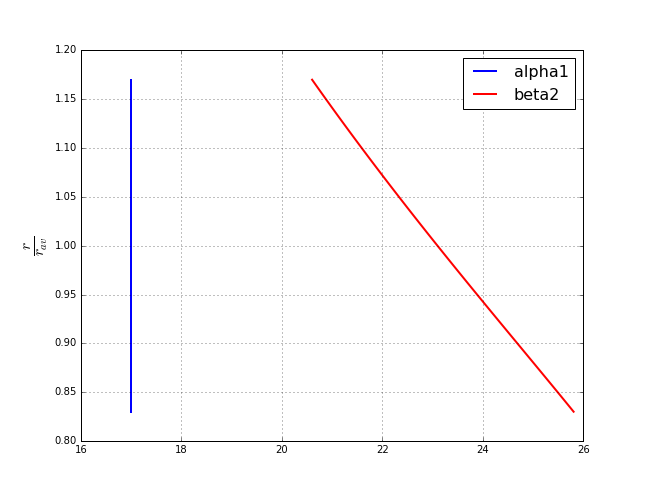
\includegraphics[scale=0.3]{../../plots/alpha1_beta2_st1.png}
\caption{Изменение углов $\alpha_1$ и $\beta_2$ по радиусу}
\end{figure}

\begin{figure}[hbtp]
\centering
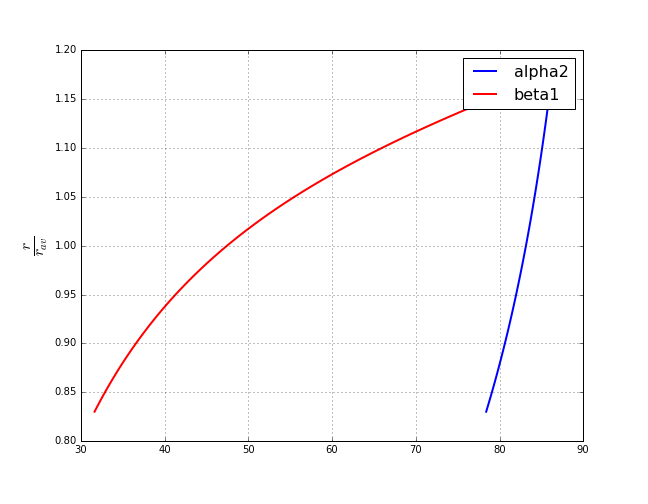
\includegraphics[scale=0.3]{../../plots/alpha2_beta1_st1.png}
\caption{Изменеие углов $\alpha_2$ и $\beta_1$ по радиусу}
\end{figure}

\begin{figure}[hbtp]
\centering
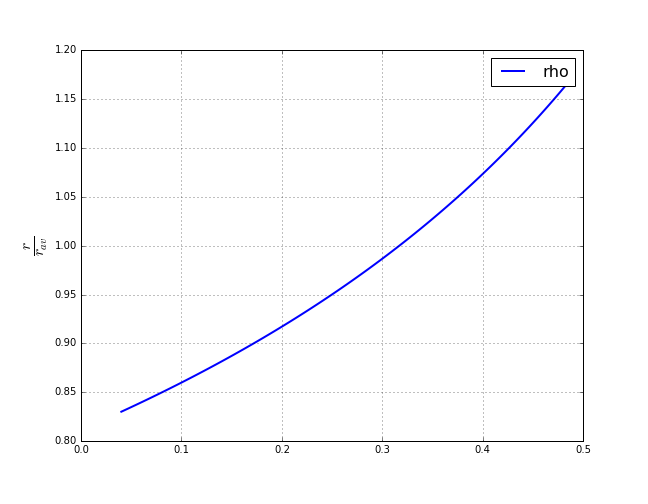
\includegraphics[scale=0.3]{../../plots/rho_st1.png}
\caption{Изменение степени реактивности по радиусу}
\end{figure}

\begin{figure}[hbtp]
\centering
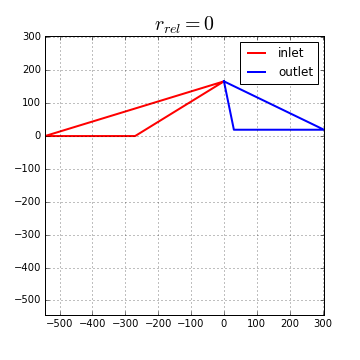
\includegraphics[scale=0.5]{../../plots/st1_triangles_0.png}
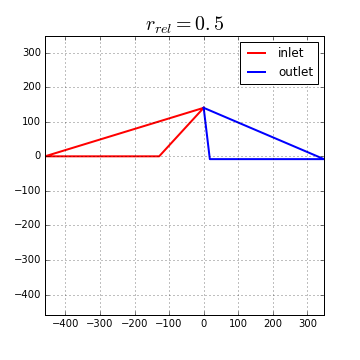
\includegraphics[scale=0.5]{../../plots/st1_triangles_1.png}
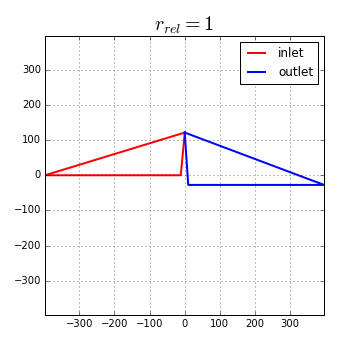
\includegraphics[scale=0.5]{../../plots/st1_triangles_2.png}
\caption{Треугольники скоростей}
\end{figure}


\section{Расчет на прочность диска первой ступени}
\subsection{Исходные данные для расчета}
\begin{enumerate}
\item Частота вращения: $n = <AngVelocity>\ об/мин$
\item Зависимость толщины диска от радиуса: $h\left( r \right)$
\item Сила инерции, действующая на лопатку: $P_{лоп} = <BladeForce>\ Н$
\item Ширина хвостовика: $h_{m-1} = <TailWidth>\ м$
\item Радиусы хвостовика: $r1 = <TailR1>\ м$ и $r2 = <TailR2>\ м$
\item Температура на внутреннем радиусе: $T_1 = 200\ К$
\item Температура на внешенм радиусе: $T_m = <OutTemp>\ К$
\item Закон изменения температуры диска по радиусу: 
Примем, что температура диска изменяется по радиусу по закону квадратной параболы:
\[T\left( r \right) = T_1 + \left( T_m - T_1 \right) \frac{r}{r_m} ^2\]
\item Число лопаток: $z_{л} = <BladeNumber>$
\item Параметры материала:

\begin{enumerate}
	\item Материал - сплав ЭИ698.
	\item Плотность: $\rho = <Density> кг/м^3$
	\item Коэффициент Пуассона: $\mu = 0.3$
	\item Зависимость модуля Юнга от температуры:
	
	\begin{tabular}{|c|c|c|c|c|c|c|}
	\hline 
	T, К & 20 & 400 & 500 & 600 & 700 & 800 \\ 
	\hline 
	E, МПа & $2\cdot10^5$ & $1.82\cdot10^5$ & $1.75\cdot10^5$ & $1.65\cdot10^5$ & $1.55\cdot10^5$ & $1.4\cdot10^5$ \\ 
	\hline 
	\end{tabular} 
	
	\item Зависимость коэффициента линейного раширения от температруы
	
	\begin{tabular}{|c|c|c|c|c|c|c|c|c|c|}
	\hline 
	T, К & 100 & 200 & 300 & 400 & 500 & 600 & 700 & 800 & 900 \\ 
	\hline 
	$\alpha, 10^{-6} 1/К$ & 11 & 11.4 & 11.7 & 12.1 & 12.4 & 12.7 & 13.4 & 13.9 & 14.7 \\ 
	\hline 
	\end{tabular} 
	
	\item Зависимость предела временной прочности от температуры
	
	\begin{tabular}{|c|c|c|c|c|c|}
		\hline 
		T, К & 20 & 400 & 500 & 600 & 700 \\ 
		\hline 
		$\sigma_в, МПа$ & 1220 & 1180 & 1160 & 1120 & 1040 \\ 
		\hline 
		\end{tabular} 	
	
\end{enumerate}
\end{enumerate}

\subsection{Алгоритм расчета}
\begin{enumerate}
\item Определяем силу нагрузку на периферии:
\[p_m = \frac{P_{лоп} z_{л}}{2 \pi r_{2} h_{m-1}} + 
  \rho \left( \frac{\pi n}{30} \right)^2 \frac{r_2^3 - r_1^3}{3 r_1} = 
  \frac{<BladeForce> \cdot <BladeNumber>}{2 \pi  \cdot <TailR2> \cdot <TailWidth>} + 
  <Density> \cdot \left( \frac{\pi \cdot <AngVelocity>}{30} \right)^2 \frac{ <TailR2>^3 -  <TailR1>^3}{3  <TailR1>} = <OutPressure>\ МПа\]
 \item Разобьем диск на $m-1$ участков постоянной толщины.
 \item Зададим значение $\sigma_r^{1,1} = \sigma_t^{1,1}=100..200\ МПа$
 \item Длякаждого из участков решим следующую систему уравнений:
 \begin{equation*}
 \begin{cases}
 S_{i,i} = \sigma_r^{i,i} + \sigma_t^{i,i}, 
 \\
 D_{i,i} = \sigma_r^{i, i} - \sigma_t^{i,i},
 \\
 S_{i,i+1} =  S_{i,i} - \frac{1+ \mu}{2}\rho_i \omega^2 
 \left( r_{i+1}^2 - r_i^2 \right) - E_i \left( \theta_{i+1} - \theta_i \right),
 \\
  D_{i, i+1} = D_{i, i} \frac{r_i^2}{r_{i+1}^2} + \frac{1- \mu}{4} \rho \omega^2 \left( r_{i+1} ^2 - \frac{r_i^4}{r_{i+1}^2} \right) + 
  2 \frac{E_i}{r_{i+1}^2} \int\limits_{r_i}^{r_{i+1}}\theta r dr - E_{i} \left(
  \theta_{i+1} - \theta_i \frac{r_i^2}{r_{i+1}^2} \right),
  \\
\sigma_t^{i, i+1} = \frac{S_{i,i+1} + D_{i,i+1}}{2},
\\
\sigma_r^{i, i+1} = \frac{S_{i,i+1} - D_{i,i+1}}{2},
\\
\sigma_r^{i+1, i+1} = \sigma_r^{i, i+1} \frac{h_i}{h_{i+1}},
\\
\sigma_t^{i+1, i+1} = \mu \sigma_t^{i, i+1} \frac{h_i}{h_{i+1}} + 
\frac{E_{i+1}}{E_i} \left(\sigma_t^{i,i+1} - \mu \sigma_r^{i, i+1} \right),
 \end{cases} 
 \end{equation*}
 где $\theta \left( r_i \right) = \alpha \left( r_i \right)  
 \left( T\left( r_i \right) - T_0 \right)$ - температурные деформации, а $T_0 = 20^\circ C$
 \item Повторяем пукты 3 и 4 при $\theta=0$ и $\omega = 0$
 \item Находим коэффициент $k$:
 \[k = \frac{p_m - (\sigma_r^{m-1, m})_I}{(\sigma_r^{m-1, m})_{II}}\]
 \item Находим значения напряжений на каждом из участков:
 \[\sigma_r^{i,j} = (\sigma_r^{i,j})_I + k(\sigma_r^{m-1, m})_{II}\]
 \[\sigma_t^{i,j} = (\sigma_t^{i,j})_I + k(\sigma_t^{m-1, m})_{II}\]
\end{enumerate}

\subsection{Результаты расчета}
\begin{enumerate}

\item Результаты первого расчета.

\begin{center}
\begin{tabular}{|c|c|c|c|}
\hline 
$i$ & $r_i,\ мм$ & $\sigma_r^{i,j},\ МПа$ & $\sigma_t^{i,j},\ МПа$ \\ 
\hline 

<FirstCalculationRows>
\end{tabular} 
\end{center}

\item Результаты второго расчета

\begin{center}
\begin{tabular}{|c|c|c|c|}
\hline 
$i$ & $r_i,\ мм$ & $\sigma_r^{i,j},\ МПа$ & $\sigma_t^{i,j},\ МПа$ \\ 
\hline 

<SecondCalculationRows>
\end{tabular} 
\end{center}

\item Значение коэффициента $k$:
\[k = \frac{p_m - (\sigma_r^{m-1, m})_I}{(\sigma_r^{m-1, m})_{II}} = 
\frac{<OutPressure> - <SigmaRKFirst>}{<SigmaRKSecond>} = <RecalculationCoef>\]

\item Значения напряжений на участках после пересчета.

\begin{center}
\begin{tabular}{|c|c|c|c|}
\hline 
$i$ & $r_i,\ мм$ & $\sigma_r^{i,j},\ МПа$ & $\sigma_t^{i,j},\ МПа$ \\ 
\hline 

<RealStressRows>
\end{tabular} 
\end{center}

\item Средние арифметические значения напряжений на радиусах

\begin{center}
\begin{tabular}{|c|c|c|c|c|}
\hline 
$i$ & $r_i,\ мм$ & $\sigma_r^{i},\ МПа$ & $\sigma_t^{i},\ МПа$ & $\sigma_{экв}^i$ \\ 
\hline 
<AverageStressRows>
\end{tabular} 
\end{center}

\item Максимальная величина эквивалентных напряжений:
\[\sigma_{экв}^i = \sqrt{(\sigma_1^i)^2 + (\sigma_3^i)^2 - \sigma_1^i \sigma_3^i}\]
\[\sigma_{экв\ мах} = <MaxEqSigma>\ МПа\]
\item Минимальный коэффициент запаса по временной прочности:
\[n_{в min} = <MinSafetyFactor>\]
\item Коэффициенты концентраций напряжений у отверстий:
\[k_1 = 3 - \frac{d_1}{b_1} - \frac{\sigma_{r1}}{\sigma_{t1}} = 
3 - \frac{<DHole1>}{<BHole1>} - \frac{<SigmaRHole1>}{<SigmaTHole1>} = <KHole1>\]
\[k_2 = 3 - \frac{d_2}{b_2} - \frac{\sigma_{r2}}{\sigma_{t2}} = 
3 - \frac{<DHole2>}{<BHole2>} - \frac{<SigmaRHole2>}{<SigmaTHole2>} = <KHole2>\]
\item Напряжения в зонах концентрации:
\[\sigma_{tк1} = k_1 \sigma_{t1} = <KHole1> \cdot <SigmaTHole1> = <SigmaTKHole1>\]
\[\sigma_{tк2} = k_2 \sigma_{t2} = <KHole2> \cdot <SigmaTHole2> = <SigmaTKHole2>\]
\item Зависимотb от радиуса радиальных, окружных и эквивалентных напряжений, а также коэффициента запаса по временной прочности.
\begin{figure}[hbtp]
\centering
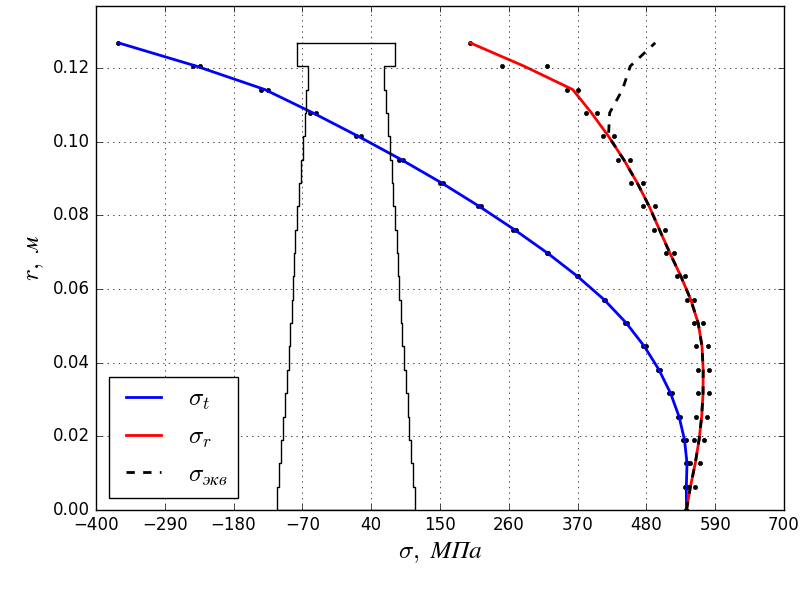
\includegraphics[scale=0.7]{../../strength_calculation/output/StressPlot.png}
\caption{Зависимость напряжений от радиуса}
\end{figure}
\begin{figure}[hbtp]
\centering
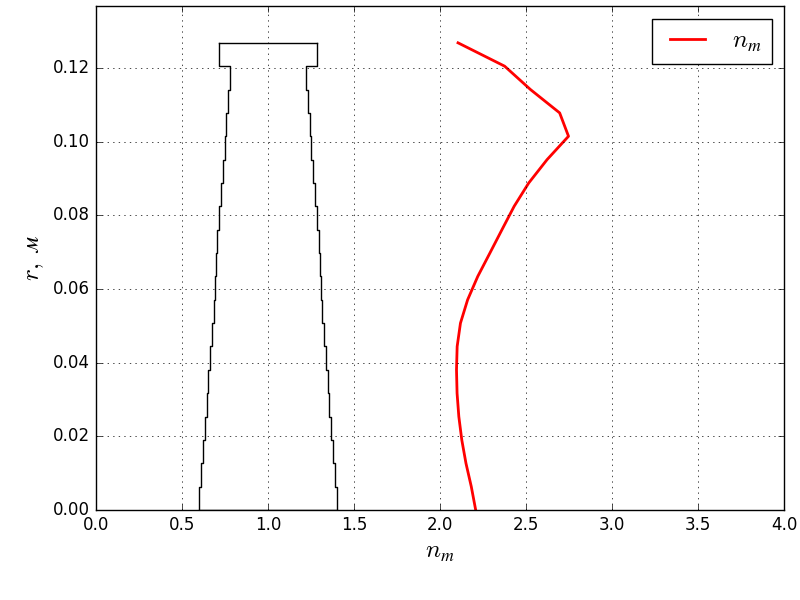
\includegraphics[scale=0.7]{../../strength_calculation/output/SafetyFactorPlot.png}
\caption{Зависимость коэффициента запаса от радиуса}
\end{figure}

\end{enumerate}
\end{document}
